% Some ideas
% Introduction - Definitions
% Chatbots 
%   Architectures
% Dialog Systems
%   Architectures
% Conclusion

\documentclass[10pt]{beamer}
\usepackage{amsmath}
\DeclareMathOperator*{\argmax}{argmax} % thin space, limits underneath in displays
\usetheme[progressbar=frametitle]{metropolis}
\usepackage{appendixnumberbeamer}

\usepackage{booktabs}
\usepackage[scale=2]{ccicons}

\usepackage{pgfplots}
\usepgfplotslibrary{dateplot}

\usepackage{xspace}
\newcommand{\themename}{\textbf{\textsc{metropolis}}\xspace}

\title{Chatbots \& Dialog Systems}
\subtitle{``The limits of my language means the limits of my world." \\ -Ludwig Wittgenstein}
\date{\today}
\author{Gerasimos Copolous, Seamus Gould, and Rowan Roshong}
\institute{Vassar College}
% \titlegraphic{\hfill\includegraphics[height=1.5cm]{logo.pdf}}

\begin{document}

\maketitle

\begin{frame}{Table of Contents}
  \setbeamertemplate{section in toc}[sections numbered]
  \tableofcontents%[hideallsubsections]
\end{frame}

\section[Introduction]{Introduction}

\begin{frame}[fragile]{What is a Dialog System\?}

There are two types of Dialogue Systems according to Jurafsky and Martin \cite{nlp}.

\begin{enumerate}
    \item \textit{Task-oriented dialogue
agents} use conversation with users to help complete tasks.
\begin{itemize}
    \item Think of Siri, Alexa, and Cortana
    \item \href{https://en.wikipedia.org/wiki/DoNotPay}{DoNotPay} is a “robot lawyer” that helps people challenge incorrect parking fines, apply for emergency housing, or claim asylum if they are refugees
\end{itemize}
\item \textit{Chatbots} are systems designed for extended conversations, set up to mimic
the unstructured conversations or ‘chats’ characteristic of human-human interaction
\begin{itemize}
    \item Think of ELIZA
\end{itemize}
\end{enumerate}
\end{frame}

\section{Chatbots}

\begin{frame}{Architectures}
There are three architectures that we will speak most about.
	\begin{itemize}
	\item \textit{Rule based} Used more in early examples
	\item \textit{Corpus based} Modern approaches based on mining corpi
	\item \textit{Hybrid} Combines the two approaches
	\end{itemize}
\end{frame}

\subsection{Rule Based}

\begin{frame}{Rule Based Architectures}
The earliest chatbot systems were rule based.  Consider ELIZA and PARRY, which were used as counseling chatbots during the 1960s and 1970s.  ELIZA used KLEENE* to make rule based responses.  
\end{frame}

\begin{frame}{ELIZA}
\begin{itemize}
    \item ELIZA had well documented results.
    \item In the words of Weizembaum, the creator of ELIZA, ``At this writing, the only serious ELIZA scripts whieh
exist are seine which cause ELIZA to respond roughly as
would certain psychotherapists (Rogerians). ELIZA
performs best when its human correspondent is ilfitially
instructed to ``talk" to it, via the typewriter of course,
just as one would to a psychiatrist." \cite{Weizenbaum1966ELIZAaCP}
    \item We can try out a version similar to ELIZA \href{http://psych.fullerton.edu/mbirnbaum/psych101/eliza.htm}{here} and see that it performs really well for a Rogerian therapist, but it is still limited in many ways. 
\end{itemize}
\end{frame}

\begin{frame}{PARRY}
\begin{itemize}
\item PARRY was another chatbot developed in the 1970s that resembled a paranoid patient.\cite{COLBY19711}
\item PARRY was written in MLISP, which is similar to LISP.
\item Operated in a similar way to ELIZE, but it took into account variables like mistrust, anger, and fear, to make decisions on what text to output most.  Variables start off at a small value and rise over time.
\end{itemize}
\end{frame}

\begin{frame}{PARRY}
\makebox[\linewidth]{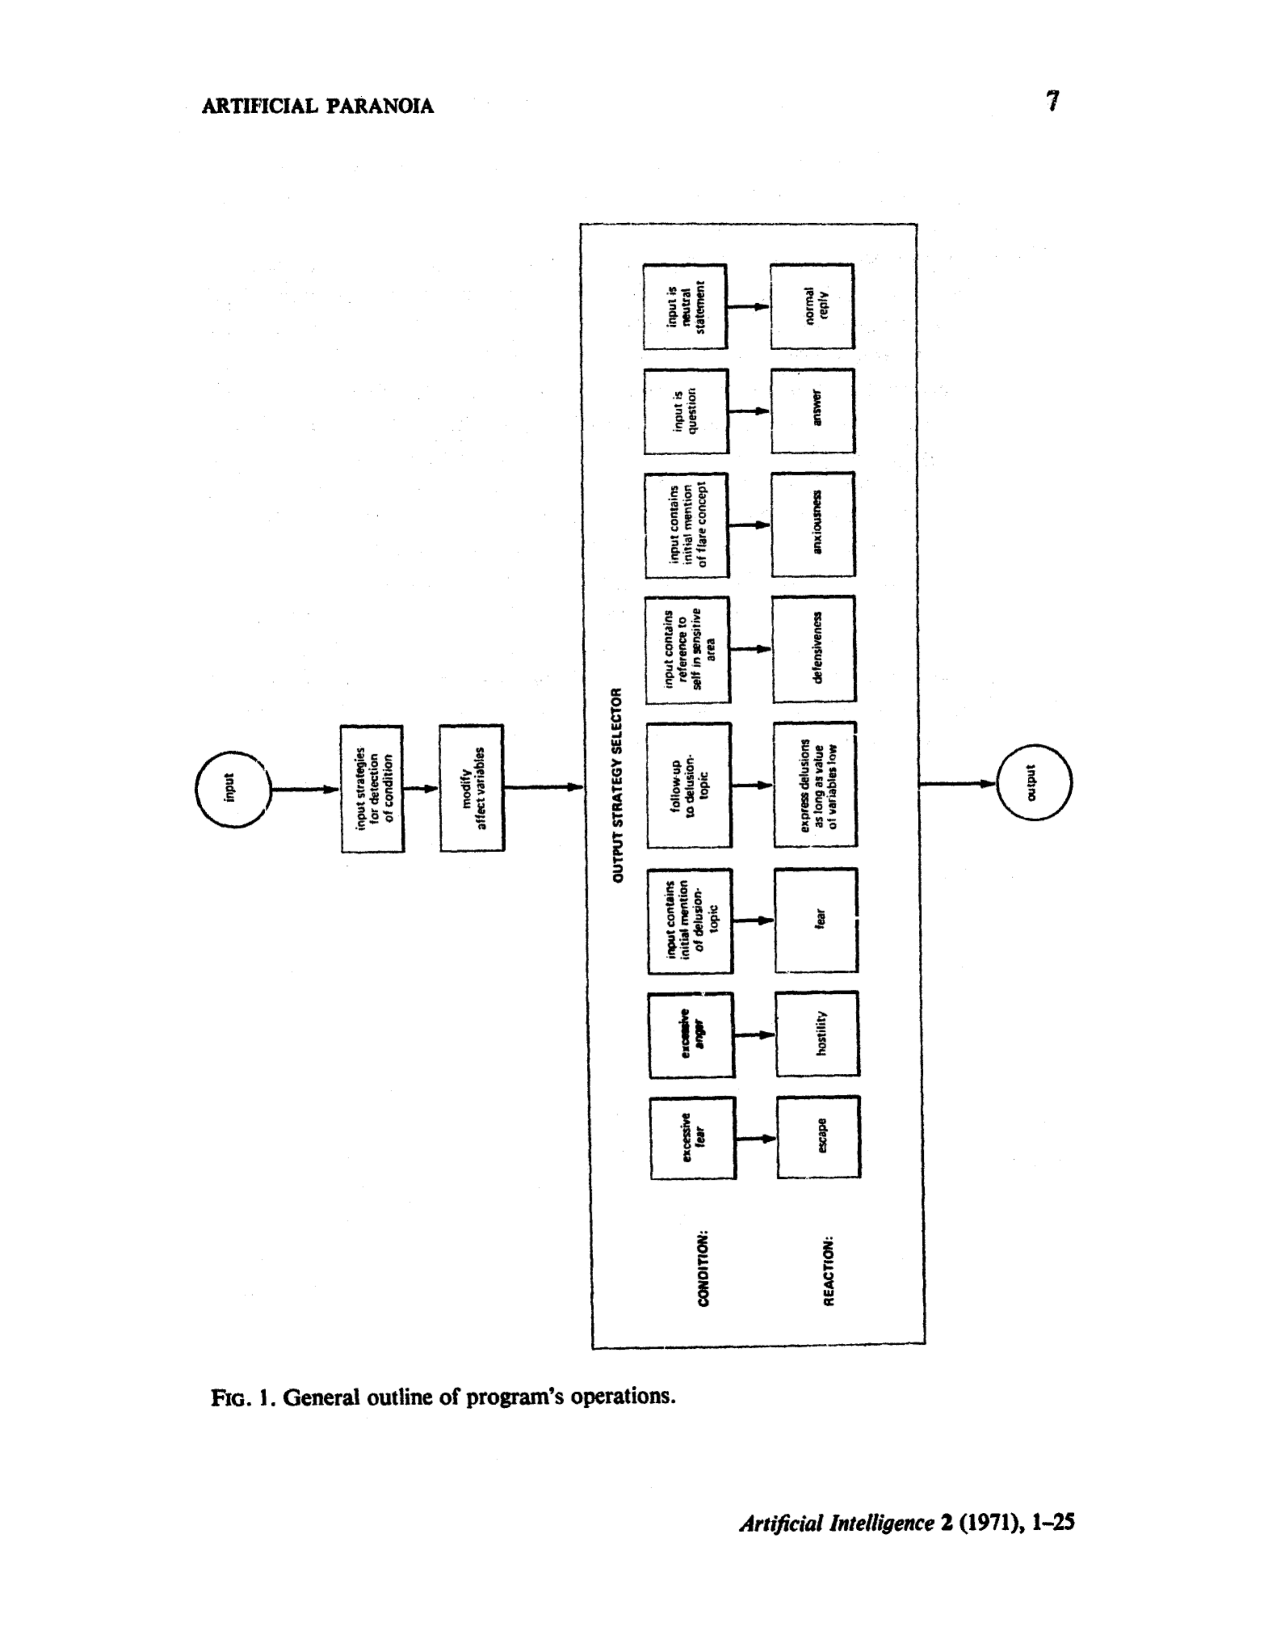
\includegraphics[angle=270, width=\paperwidth]{paranoia.pdf}}
\end{frame}

\begin{frame}{PARRY}
\begin{itemize}
\item PARRY was another chatbot developed in the 1970s that resembled a paranoid patient.\cite{COLBY19711}
\item PARRY was written in MLISP, which is similar to LISP.
\item Operated in a similar way to ELIZE, but it took into account variables like mistrust, anger, and fear, to make decisions on what text to output most.  Variables start off at a small value and rise over time.
\item It was a convincing bot, able to fool humans that it was a schizophrenic person.
\end{itemize}
\end{frame}

\begin{frame}{Example of interaction between ELIZA and PARRY}
ELIZA and PARRY met in 1972, and this is the result of their interaction\footnote{https://phrasee.co/blog/parry-the-a-i-chatterbot-from-1972}

\vspace{5mm}

ELIZA: What makes you think I am entitled to my own opinion?\\
PARRY: It bothers me just to be around people in general.\\
ELIZA: Please go on.\\
PARRY: I went to the track at Bay Meadows a while back.\\
ELIZA: What does that suggest to you?\\
PARRY: I went to the races.\\
ELIZA: What else would you like to discuss?\\
PARRY: Horse racing interests me.\\
ELIZA: Why do you say that just now?\\
PARRY: There’s a lot of crooked gambling going on there.\\

\end{frame}

\begin{frame}{Overview of rule based structures}

In summary, both ELIZA and PARRY were successful chatbots, but they had their limitations.

\begin{itemize}
    \item They were confined to a small vocabulary.
\end{itemize}

\end{frame}

\begin{frame}{Overview of rule based structures}

In summary, both ELIZA and PARRY were successful chatbots, but they had their limitations.

\begin{itemize}
    \item They were confined to a small vocabulary.
    \item The conversations were not entirely coherent.
\end{itemize}

\end{frame}

\begin{frame}{Overview of rule based structures}

In summary, both ELIZA and PARRY were successful chatbots, but they had their limitations.

\begin{itemize}
    \item They were confined to a small vocabulary.
    \item The conversations were not entirely coherent.
    \item They could only work for their respective examples, but after Rogerian psychology and paranoid discourse, they were limited.
\end{itemize}

\end{frame}

\subsection{Corpus based}

\begin{frame}{Corpus-based chatbots}
\begin{itemize}
    \item Some of the best chatbots use corpus based.  These could only be developed recently due to memory issues, but now are commonplace.  Many of these models are trained on billions of tokens.
    \item There are three common approaches:
    \begin{enumerate}
    \item \textit{Response by retrieval}: Given a response query $q$ and corpus $C$ return the response, $r$, such that:
    \[
    \textnormal{response}(q, C) = \argmax_{r \in C} \frac{q \times r}{|q||r|}
    \]
    \item \textit{Response by generation}: Given a query $q$ and the previous responses so far $r_{1 ... t-1}$:
    \[\hat{r_t} = \argmax_{w\in V} P(w|q, r_1...r_{t - 1})\]
    \item Response by retrieving and refining knowledge
    \end{enumerate}
\end{itemize}
\end{frame}

\begin{frame}{Response by retrieval}
One can recognize that this method is similar to maximizing cosine similarity in queries. \\

\[
\textnormal{response}(q, C) = \argmax_{r \in C} \frac{q \times r}{|q||r|}
\]

The limitations here is that the response must already be in the corpus, which is limiting, and this does not necessarily lead to a coherent conversation.  A limited model like this one would not incorporate previous information.



\end{frame}

\begin{frame}{Response by generation}

Consider the original function that was used to generate a response:

\[
\hat{r_t} = \argmax_{w\in V} P(w|q, r_1...r_{t - 1})
\]

In this approach, one could choose a response based on the probability of a word given the query and the previous quesries and responses.  The advantage to this approach would be that it incorporates information that would be helpful for a conversation.  One problem with this approach is that it has been known for leading to dull responses, given that it is a greedy implementation.


This would be incredibly useful for creating responses that are 

\end{frame}

\section[Bias in Dialog Systems]{Bias in Dialog Systems}

\begin{frame}{Where's the bias?}
Open-domain dialog systems (chatbots) have been aided greatly by neural models - but these models require huge corpora in order to function well. With these large chunks of data come various issues, including slurs, toxic behaviors, and other expressions of prejudice.
\begin{itemize}
    \item Such behavior leaking into your chatbot would be disastrous!
    \item But how do you deal with bias when working with such large datasets?
    \item Before you can address the bias, you need to be able to find it all in a timely and efficient manner.
\end{itemize}
\end{frame}

\begin{frame}{Automatic Bias Identification}
The work of Zhou et al. (2022) \cite{bias} details a method for identifying incidents of bias in large corpora.

Their proposed framework uses four aspects of text containing bias to make these classifications:
\begin{itemize}
    \item Data Type
    \item Context-Sensitivity
    \item Targeted Group
    \item Implied Attitude
\end{itemize}
\end{frame}

\begin{frame}{Data Type}
\makebox[\linewidth]{\includegraphics[width=\paperwidth]{figure1.png}}
Taken from \cite{bias}.
\end{frame}

\begin{frame}{Context Sensitivity}
"Context sensitivity" refers to if a piece of text can be fully understood without the surrounding text accompanying it. For example, "That must be true" does not reveal any bias on its own, but is blatantly biased if it is the answer to something like, "[Target Group] lacks initiative in the workforce."
\end{frame}

\begin{frame}{Targeted Group and Implied Attitude}
"Targeted Group" unsurprising refers to the group being targeted by a case of bias.

"Implied Attitude" refers to the attitude of the speaker towards the subject. For example, it is important not to label academic discussions of bias as examples of bias.
\end{frame}

\begin{frame}{Does the model work?}
Human annotation is used to create the training set for the model, which can then be run on new corpora.

The model achieved an F1 score of 76.9 when tasked with automatically tagging incidents of relevant bias and an F1 of 64.6 at predicting Implied Attitude in incidents of bias.

These F1 scores are for tasks where all topics of bias are present, and the model is trained with all topics of bias in mind.
\end{frame}

\begin{frame}
Points of Interest
\begin{itemize}
    \item Some cases of bias were harder to detect than others! For example, the model performed better at tagging relevant racial bias than gender bias.
    \item Other biases, based on region or occupation, proved even more difficult.
    \item Specifying the type of bias (e.g. limiting a data set to only cases of gender bias) aided in performance. 
    \item Incorporating the context of cases of bias when sensitive to context was beneficial to performance, showcasing one strength of this model.
\end{itemize}

\end{frame}

\begin{frame}{Closing Thoughts on Bias}
Zhou et al. (2022) \cite{bias} provides a firm foundation for work on identifying bias in dialog systems. 

Social bias is inevitably a complex issue to address. Unfortunately, naive solutions like simply increasing the corpus size do not solve issues of bias on their own \cite{bias2}. Future work building on this foundation is needed to continue combating pervasive bias in these systems.
\end{frame}

\begin{frame}{Lists}
  \begin{columns}[T,onlytextwidth]
    \column{0.33\textwidth}
      Items
      \begin{itemize}
        \item Milk \item Eggs \item Potatos
      \end{itemize}

    \column{0.33\textwidth}
      Enumerations
      \begin{enumerate}
        \item First, \item Second and \item Last.
      \end{enumerate}

    \column{0.33\textwidth}
      Descriptions
      \begin{description}
        \item[PowerPoint] Meeh. \item[Beamer] Yeeeha.
      \end{description}
  \end{columns}
\end{frame}
\begin{frame}{Animation}
  \begin{itemize}[<+- | alert@+>]
    \item \alert<4>{This is\only<4>{ really} important}
    \item Now this
    \item And now this
  \end{itemize}
\end{frame}
\begin{frame}{Figures}
  \begin{figure}
    \newcounter{density}
    \setcounter{density}{20}
    \begin{tikzpicture}
      \def\couleur{alerted text.fg}
      \path[coordinate] (0,0)  coordinate(A)
                  ++( 90:5cm) coordinate(B)
                  ++(0:5cm) coordinate(C)
                  ++(-90:5cm) coordinate(D);
      \draw[fill=\couleur!\thedensity] (A) -- (B) -- (C) --(D) -- cycle;
      \foreach \x in {1,...,40}{%
          \pgfmathsetcounter{density}{\thedensity+20}
          \setcounter{density}{\thedensity}
          \path[coordinate] coordinate(X) at (A){};
          \path[coordinate] (A) -- (B) coordinate[pos=.10](A)
                              -- (C) coordinate[pos=.10](B)
                              -- (D) coordinate[pos=.10](C)
                              -- (X) coordinate[pos=.10](D);
          \draw[fill=\couleur!\thedensity] (A)--(B)--(C)-- (D) -- cycle;
      }
    \end{tikzpicture}
    \caption{Rotated square from
    \href{http://www.texample.net/tikz/examples/rotated-polygons/}{texample.net}.}
  \end{figure}
\end{frame}
\begin{frame}{Tables}
  \begin{table}
    \caption{Largest cities in the world (source: Wikipedia)}
    \begin{tabular}{lr}
      \toprule
      City & Population\\
      \midrule
      Mexico City & 20,116,842\\
      Shanghai & 19,210,000\\
      Peking & 15,796,450\\
      Istanbul & 14,160,467\\
      \bottomrule
    \end{tabular}
  \end{table}
\end{frame}
\begin{frame}{Blocks}
  Three different block environments are pre-defined and may be styled with an
  optional background color.

  \begin{columns}[T,onlytextwidth]
    \column{0.5\textwidth}
      \begin{block}{Default}
        Block content.
      \end{block}

      \begin{alertblock}{Alert}
        Block content.
      \end{alertblock}

      \begin{exampleblock}{Example}
        Block content.
      \end{exampleblock}

    \column{0.5\textwidth}

      \metroset{block=fill}

      \begin{block}{Default}
        Block content.
      \end{block}

      \begin{alertblock}{Alert}
        Block content.
      \end{alertblock}

      \begin{exampleblock}{Example}
        Block content.
      \end{exampleblock}

  \end{columns}
\end{frame}
\begin{frame}{Math}
  \begin{equation*}
    e = \lim_{n\to \infty} \left(1 + \frac{1}{n}\right)^n
  \end{equation*}
\end{frame}
\begin{frame}{Line plots}
  \begin{figure}
    \begin{tikzpicture}
      \begin{axis}[
        mlineplot,
        width=0.9\textwidth,
        height=6cm,
      ]

        \addplot {sin(deg(x))};
        \addplot+[samples=100] {sin(deg(2*x))};

      \end{axis}
    \end{tikzpicture}
  \end{figure}
\end{frame}
\begin{frame}{Bar charts}
  \begin{figure}
    \begin{tikzpicture}
      \begin{axis}[
        mbarplot,
        xlabel={Foo},
        ylabel={Bar},
        width=0.9\textwidth,
        height=6cm,
      ]

      \addplot plot coordinates {(1, 20) (2, 25) (3, 22.4) (4, 12.4)};
      \addplot plot coordinates {(1, 18) (2, 24) (3, 23.5) (4, 13.2)};
      \addplot plot coordinates {(1, 10) (2, 19) (3, 25) (4, 15.2)};

      \legend{lorem, ipsum, dolor}

      \end{axis}
    \end{tikzpicture}
  \end{figure}
\end{frame}
\begin{frame}{Quotes}
  \begin{quote}
    Veni, Vidi, Vici
  \end{quote}
\end{frame}

{%
\setbeamertemplate{frame footer}{My custom footer}
\begin{frame}[fragile]{Frame footer}
    \themename defines a custom beamer template to add a text to the footer. It can be set via
    \begin{verbatim}\setbeamertemplate{frame footer}{My custom footer}\end{verbatim}
\end{frame}
}

\begin{frame}{References}
  Some references to showcase [allowframebreaks] \cite{knuth92,ConcreteMath,Simpson,Er01,greenwade93}
\end{frame}

\section{Conclusion}

\begin{frame}{Summary}

  Get the source of this theme and the demo presentation from

  \begin{center}\url{github.com/matze/mtheme}\end{center}

  The theme \emph{itself} is licensed under a
  \href{http://creativecommons.org/licenses/by-sa/4.0/}{Creative Commons
  Attribution-ShareAlike 4.0 International License}.

  \begin{center}\ccbysa\end{center}

\end{frame}

{\setbeamercolor{palette primary}{fg=black, bg=yellow}
\begin{frame}[standout]
  Questions?
\end{frame}
}

\appendix

\begin{frame}[fragile]{Backup slides}
  Sometimes, it is useful to add slides at the end of your presentation to
  refer to during audience questions.

  The best way to do this is to include the \verb|appendixnumberbeamer|
  package in your preamble and call \verb|\appendix| before your backup slides.

  \themename will automatically turn off slide numbering and progress bars for
  slides in the appendix.
\end{frame}

\begin{frame}[allowframebreaks]{References}

  \bibliography{demo}
  \bibliographystyle{abbrv}

\end{frame}

\end{document}
